\documentclass[conference]{IEEEtran}
\IEEEoverridecommandlockouts
% The preceding line is only needed to identify funding in the first footnote. If that is unneeded, please comment it out.
\usepackage{cite}
\usepackage{amsmath,amssymb,amsfonts}
\usepackage{algorithmic}
\usepackage{graphicx}
\usepackage{textcomp}
\usepackage{xcolor}
\usepackage{tabularx}
\usepackage{multirow}
\usepackage{graphics} % for pdf, bitmapped graphics files
\usepackage{subfig}
\usepackage{subcaption}
\usepackage{hyperref}
\usepackage{academicons}
\usepackage{xcolor}
\usepackage{tabularx} % Asegúrate de incluir este paquete

% minted for use pygmetize
\usepackage{minted}
\usepackage{geometry}            % Márgenes
\usepackage{courier}			 % font type

% Opciones globales (opcional) minted
\setminted{
	frame=lines,                 % Marco superior e inferior
	framesep=2mm,                % Espaciado del marco
	baselinestretch=1.1,         % Espaciado entre líneas
	fontsize=\small,     		 % Tamaño de fuente
	linenos,                     % Números de línea
	breaklines,                  % Saltar líneas largas
	bgcolor=gray!5,              % Fondo gris claro
	tabsize=4,                   % Tamaño de tabulación
	autogobble,                  % Ajusta indentación automáticamente
	xleftmargin=1em,             % Margen izquierdo,
	fontfamily=pcr
}

% config colores to minted
\definecolor{bg}{rgb}{0.95,0.95,0.95}
\definecolor{keyword}{rgb}{0.13,0.13,1}
\definecolor{comment}{rgb}{0.25,0.5,0.35}
\definecolor{string}{rgb}{0.58,0,0.13}
\definecolor{bgdark}{HTML}{2D2D2D}

\usepackage{tikz}
\usetikzlibrary{shapes.geometric, arrows}

\usetikzlibrary{shapes.geometric, arrows}

\tikzstyle{startstop} = [rectangle, rounded corners, minimum width=3cm, minimum height=1cm,text centered, draw=black, fill=red!30]
\tikzstyle{process} = [rectangle, minimum width=3cm, minimum height=1cm, text centered, draw=black, fill=blue!30]
\tikzstyle{arrow} = [thick,->,>=stealth]


\def\BibTeX{{\rm B\kern-.05em{\sc i\kern-.025em b}\kern-.08em
		T\kern-.1667em\lower.7ex\hbox{E}\kern-.125emX}}

% Color Enlace
\definecolor{colorEnlace}{RGB}{0, 0, 0}
\hypersetup{
	colorlinks=true,
	linkcolor=colorEnlace,
	citecolor=colorEnlace,
	urlcolor=colorEnlace,
	pdfauthor={Equipo cero},
	pdftitle={Rectificador monofasico controlado}
}

% Control 
\usepackage{amsmath}
\begin{document}
	
	\title{Transmisión de datos mediante TDM}
	\author{
		\makebox[\textwidth][c]{\large\textbf{Universidad Nacional de San Antonio Abad del Cusco}}\\
		\makebox[\textwidth][c]{\normalsize\textit{Escuela profesional de Ingeniería Electrónica}}\\
		\makebox[\textwidth][c]{\normalsize\textit{Telecomunicaciones II}}\\
		\and
		\IEEEauthorblockN{Alexander Palomino Lopez}
		\IEEEauthorblockA{Ingeniero Electrónico \\
			Cusco, Perú \\
			alexander.palomino@unsaac.edu.pe}
		\and
		\IEEEauthorblockN{Davis Bremdow Salazar Roa - 200353}
		\IEEEauthorblockA{Estudiante de Ingeniería Electrónica \\
			Cusco, Perú \\
			200353@unsaac.edu.pe}
	}
	
	\maketitle
	\begin{abstract}
		
	\end{abstract}
	\begin{IEEEkeywords}
		
	\end{IEEEkeywords}
	
	\section{Introducción}
	\section{\textbf{Circuito detector de cruce por cero}}
	\subsection{\textbf{Función e importancia en los sistemas de control de potencia}}
	\section{Integrado H11AA1}
	\section{\textbf{Simulación}}
	
	Una acercamiento experimental sobre el circuito de control de potencia en cuestión se puede realizar mediante la implementación digital y/o simulación del circuito, usando para este fin el software de simulación \textbf{Proteus} en su versión 13.7 SP2 la cual permite el añadido de librerías para representar cada componente electrónico en su entorno, así como el uso de Arduino u otro microcontrolador el cual se usará para establecer los tiempos de disparo del circuito.
	
	El circuito de disparo considerado para la simulación constará de las siguientes etapas:
	
	\begin{enumerate}
		\item Circuito detector de cruce por cero
		\item Circuito de control (uC)
		\item Circuito de potencia (Rectificador)
	\end{enumerate}
	
	\subsection{\textbf{Circuito detector de cruce por cero}}
	Este circuito conformado por un puente rectificador y un optoacoplador para aislar la señal de potencia del circuito de control, nos permite conocer cuando la señal inicia su excursión negativa o positiva de lo cual se puede inferir que medio ciclo de la misma ha transcurrido permitiendo aplicar un algoritmo de control mediante el sensado o detección de estos cruces para establecer el tiempo de espera para activar los tiristores modificando la señal de salida rectificada.
	
	\begin{figure}[h]
		\centering
		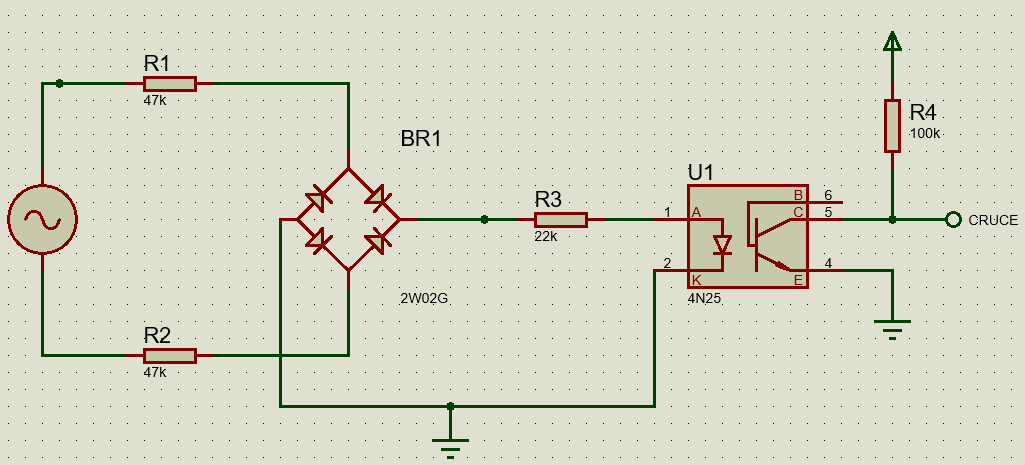
\includegraphics[width=0.5\textwidth]{media/circuito-cruce-cero}
		\caption{Circuito de cruce por cero}
		\label{fig:circuito-cruce-cero}
	\end{figure}
	
	
	En la figura \ref{fig:circuito-cruce-cero} se puede apreciar la simulación de esta primera parte del circuito de disparo.
	
	\subsection{\textbf{Circuito de control}}
	Como subsecuente elemento en la parte de control una vez verificado el correcto funcionamiento del circuito de cruce por cero como segunda parte se tiene el circuito de control conformado por el microcontrolador Arduino UNO en el cual tiene la siguiente configuración para ejecutar las acciones de control:
	
	\textbf{Pines de entrada:} \\
	\begin{enumerate}
		\item A0 (Analogica) : Para modificar el ángulo de disparo
		\item D2 (Digital/Interrupción) : Para la lectura del pulso generado por el circuito detector de cruce por cero
	\end{enumerate}
	
	\textbf{Pines de salida:}\\
	\begin{enumerate}
		\item D3 (Digital) : Para activar el tiristor SCR1 mediante un pulso
		\item D4 (Digital) : Para activar el tiristor SCR2 mediante un pulso
		\item Tx, Rx : Para la comunicación serial y uso del monitor para mostrar información de ejecución 		
	\end{enumerate}
	
	\begin{figure}[h]
		\centering
		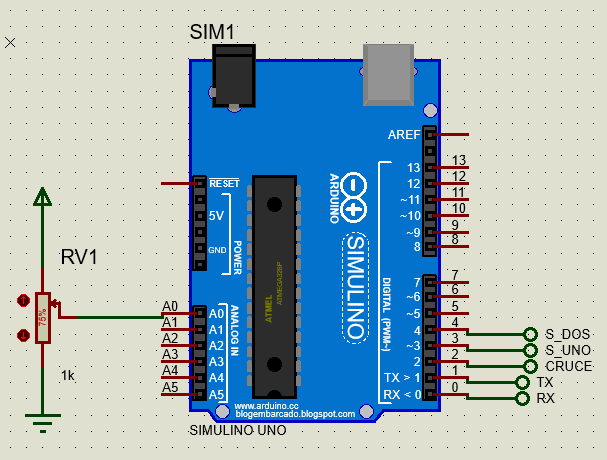
\includegraphics[width=0.5\textwidth]{media/circuito-control}
		\caption{Circuito de control - Arduino}
		\label{fig:circuito-control}
	\end{figure}
	
	En la figura \ref{fig:circuito-control} se muestra el esquema del circuito de control simulado.
	
	\subsection{\textbf{Circuito de potencia (rectificador)}}
	
	Finalmente en la etapa de potencia de salida se cuentan con los dispositivos de control como los tiristores y optotriacs como circuitos aisladores entre la etapa de control y de potencia, configurando los primeros en forma de puente para una rectificación a onda completa y colocando en primera instancia una carga resistiva, además de un osciloscopio para visualizar la forma de onda de salida en función al valor del potenciometro.
	
	
	\begin{figure}[h]
		\centering
		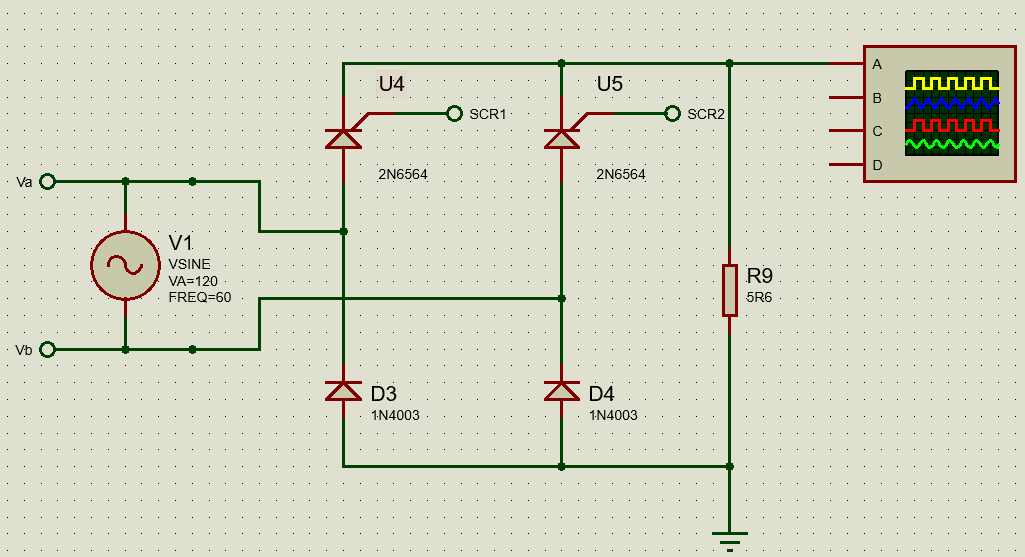
\includegraphics[width=0.5\textwidth]{media/circuito-potencia}
		\caption{Circuito de potencia - Rectificador onda completa controlado}
		\label{fig:circuito-potencia}
	\end{figure}
	
	En la figura \ref{fig:circuito-potencia} se puede apreciar el circuito de potencia implementando considerando dentro de este mismo la observación y empleo de 2 diodos rectificadores para el etapa de retorno agregados con fines de experimentación sin que esto altere en correcto funcionamiento en el circuito se implemente con dispositivos de control.
	
	\subsection{\textbf{Código Arduino}}
	
	Como anexo también se destaca el código Arduino utilizado para el control del circuito de disparo de Triacs y/o control en el rectificador monófasico de onda completa controlado, este código se muestra en el bloque \ref{lst:disparo-triac}
	
	\section{Importancia de detectar el cruce por cero en los sistemas de control}
	\section{Análisis del rectificador controlado}
	\subsection{Análisis con carga inductiva}
	\subsection{Medidas para proteger el SCR}
	
	% Resumen de lo obtenido para cada etapa
	
	% Código general aplicado y capturas de los archivos empleados para la simulación
	\bibliographystyle{IEEEtran}
	\bibliography{biblio}
	\section{Anexos}
	
	\begin{listing}
		\caption{Código de control - Disparo Tiristor}
		\label{lst:disparo-triac}
		\begin{minted}[bgcolor=bg, linenos=false, style=arduino]{c}
			
			// Variables de control
			volatile boolean cruceCero = 0;
			int triac = 3;
			int triac2 = 4;
			int x = 1;
			int POT;
			int dim;
			
			// Configuración inicial
			void setup() {
				Serial.begin(9600);
				pinMode(triac, OUTPUT);
				pinMode(triac2, OUTPUT);
				attachInterrupt(0, deteccionCruceCero, RISING);
			}
			
			void deteccionCruceCero(){
				cruceCero = true;
				x++;
				if (x == 3){
					x = 1;
				}
				Serial.println(x),
				digitalWrite(triac, LOW);
				digitalWrite(triac2, LOW);
			}
			
			void loop() {
				POT = analogRead(A0);
				dim = map(POT, 0, 1023, 0, 8.3);
				
				
				// Envía los pulsos según el valor actual del pot para el tiempo
				
				if ( x == 1 && cruceCero == true){
					delay(dim);
					digitalWrite(triac, HIGH);
					delay(1);
					digitalWrite(triac, LOW);
					cruceCero = false;
				}
				
				
				if ( x == 2 && cruceCero == true){
					delay(dim);
					digitalWrite(triac2, HIGH);
					delay(1);
					digitalWrite(triac2, LOW);
					cruceCero = false;
				}
			}
		\end{minted}
	\end{listing}
	
\end{document}